
% Template for a Computer Science Tripos Part II project dissertation
\documentclass[12pt,a4paper,twoside,openright]{report}
\usepackage[pdfborder={0 0 0}]{hyperref}    % turns references into hyperlinks
\usepackage[margin=25mm]{geometry}  % adjusts page layout
\usepackage{graphicx}  % allows inclusion of PDF, PNG and JPG images
\usepackage{verbatim}
\usepackage{docmute}   % only needed to allow inclusion of proposal.tex

\raggedbottom                           % try to avoid widows and orphans
\sloppy
\clubpenalty1000%
\widowpenalty1000%

\renewcommand{\baselinestretch}{1.1}    % adjust line spacing to make
                                        % more readable

\begin{document}

\bibliographystyle{plain}


%%%%%%%%%%%%%%%%%%%%%%%%%%%%%%%%%%%%%%%%%%%%%%%%%%%%%%%%%%%%%%%%%%%%%%%%
% Title


\pagestyle{empty}

\rightline{\LARGE \textbf{Martin Richards}}

\vspace*{60mm}
\begin{center}
\Huge
\textbf{How to write a dissertation in \LaTeX} \\[5mm]
Computer Science Tripos -- Part II \\[5mm]
St John's College \\[5mm]
\today  % today's date
\end{center}

%%%%%%%%%%%%%%%%%%%%%%%%%%%%%%%%%%%%%%%%%%%%%%%%%%%%%%%%%%%%%%%%%%%%%%%%%%%%%%
% Proforma, table of contents and list of figures

\pagestyle{plain}

\chapter*{Proforma}

{\large
\begin{tabular}{ll}
Name:               & \bf Martin Richards                       \\
College:            & \bf St John's College                     \\
Project Title:      & \bf How to write a dissertation in \LaTeX \\
Examination:        & \bf Computer Science Tripos -- Part II, July 2001  \\
Word Count:         & \bf 1587\footnotemark[1]
                      (well less than the 12000 limit)  \\
Project Originator: & Dr M.~Richards                    \\
Supervisor:         & Dr Markus Kuhn                    \\ 
\end{tabular}
}
\footnotetext[1]{This word count was computed
by \texttt{detex diss.tex | tr -cd '0-9A-Za-z $\tt\backslash$n' | wc -w}
}
\stepcounter{footnote}


\section*{Original Aims of the Project}

To write a demonstration dissertation\footnote{A normal footnote without the
complication of being in a table.} using \LaTeX\ to save
student's time when writing their own dissertations. The dissertation
should illustrate how to use the more common \LaTeX\ constructs. It
should include pictures and diagrams to show how these can be
incorporated into the dissertation.  It should contain the entire
\LaTeX\ source of the dissertation and the makefile.  It should
explain how to construct an MSDOS disk of the dissertation in
Postscript format that can be used by the book shop for printing, and,
finally, it should have the prescribed layout and format of a diploma
dissertation.


\section*{Work Completed}

All that has been completed appears in this dissertation.

\section*{Special Difficulties}

Learning how to incorporate encapulated postscript into a \LaTeX\
document on both Ubuntu Linux and OS X.
 
\newpage
\section*{Declaration}

I, [Name] of [College], being a candidate for Part II of the Computer
Science Tripos [or the Diploma in Computer Science], hereby declare
that this dissertation and the work described in it are my own work,
unaided except as may be specified below, and that the dissertation
does not contain material that has already been used to any substantial
extent for a comparable purpose.

\bigskip
\leftline{Signed [signature]}

\medskip
\leftline{Date [date]}

\tableofcontents

\listoffigures

\newpage
\section*{Acknowledgements}

This document owes much to an earlier version written by Simon Moore
\cite{Moore95}.  His help, encouragement and advice was greatly 
appreciated.

%%%%%%%%%%%%%%%%%%%%%%%%%%%%%%%%%%%%%%%%%%%%%%%%%%%%%%%%%%%%%%%%%%%%%%%
% now for the chapters

\pagestyle{headings}

\chapter{Introduction}

\section{Overview of the files}

This document consists of the following files:

\begin{itemize}
\item \texttt{makefile} --- The makefile for the dissertation and
                         Project Proposal
\item \texttt{diss.tex} --- The dissertation
\item \texttt{proposal.tex}  --- The project proposal 
\item \texttt{figs} -- A directory containing diagrams and pictures
\item \texttt{refs.bib} --- The bibliography database
\end{itemize}

\section{Building the document}

This document was produced using \LaTeXe which is based upon
\LaTeX\cite{Lamport86}.  To build the document you first need to
generate \texttt{diss.aux} which, amongst other things, contains the
references used.  This if done by executing the command:

\texttt{pdflatex diss}

\noindent
Then the bibliography can be generated from \texttt{refs.bib} using:

\texttt{bibtex diss}

\noindent
Finally, to ensure all the page numbering is correct run \texttt{pdflatex}
on \texttt{diss.tex} until the \texttt{.aux} files do not change.  This
usually takes 2 more runs.

\subsection{The makefile}

To simplify the calls to \texttt{pdflatex} and \texttt{bibtex}, 
a makefile has been provided, see Appendix~\ref{makefile}. 
It provides the following facilities:

\begin{description}

\item\texttt{make} \\
 Display help information.

\item\texttt{make proposal.pdf} \\
 Format the proposal document as a PDF.

\item\texttt{make view-proposal} \\
 Run \texttt{make proposal.pdf} and then display it with a Linux PDF viewer
 (preferably ``okular'', if that is not available fall back to ``evince'').

\item\texttt{make diss.pdf} \\
 Format the dissertation document as a PDF.

\item\texttt{make count} \\
Display an estimate of the word count.

\item\texttt{make all} \\
Construct \texttt{proposal.pdf} and \texttt{diss.pdf}.

\item\texttt{make pub} \\ Make \texttt{diss.pdf}
and place it in my \texttt{public\_html} directory.

\item\texttt{make clean} \\ Delete all intermediate files except the
source files and the resulting PDFs. All these deleted files can
be reconstructed by typing \texttt{make all}.

\end{description}


\section{Counting words}

An approximate word count of the body of the dissertation may be
obtained using:

\texttt{wc diss.tex}

\noindent
Alternatively, try something like:

\verb/detex diss.tex | tr -cd '0-9A-Z a-z\n' | wc -w/


\chapter{Preparation}

This chapter is empty!


\chapter{Implementation}

\section{Verbatim text}

Verbatim text can be included using \verb|\begin{verbatim}| and
\verb|\end{verbatim}|. I normally use a slightly smaller font and
often squeeze the lines a little closer together, as in:

{\renewcommand{\baselinestretch}{0.8}\small
\begin{verbatim}
GET "libhdr"
 
GLOBAL { count:200; all  }
 
LET try(ld, row, rd) BE TEST row=all
                        THEN count := count + 1
                        ELSE { LET poss = all & ~(ld | row | rd)
                               UNTIL poss=0 DO
                               { LET p = poss & -poss
                                 poss := poss - p
                                 try(ld+p << 1, row+p, rd+p >> 1)
                               }
                             }
LET start() = VALOF
{ all := 1
  FOR i = 1 TO 12 DO
  { count := 0
    try(0, 0, 0)
    writef("Number of solutions to %i2-queens is %i5*n", i, count)
    all := 2*all + 1
  }
  RESULTIS 0
}
\end{verbatim}
}

\section{Tables}

\begin{samepage}
Here is a simple example\footnote{A footnote} of a table.

\begin{center}
\begin{tabular}{l|c|r}
Left      & Centred & Right \\
Justified &         & Justified \\[3mm]
%\hline\\%[-2mm]
First     & A       & XXX \\
Second    & AA      & XX  \\
Last      & AAA     & X   \\
\end{tabular}
\end{center}

\noindent
There is another example table in the proforma.
\end{samepage}

\section{Simple diagrams}

Simple diagrams can be written directly in \LaTeX.  For example, see
figure~\ref{latexpic1} on page~\pageref{latexpic1} and see
figure~\ref{latexpic2} on page~\pageref{latexpic2}.

\begin{figure}
\setlength{\unitlength}{1mm}
\begin{center}
\begin{picture}(125,100)
\put(0,80){\framebox(50,10){AAA}}
\put(0,60){\framebox(50,10){BBB}}
\put(0,40){\framebox(50,10){CCC}}
\put(0,20){\framebox(50,10){DDD}}
\put(0,00){\framebox(50,10){EEE}}

\put(75,80){\framebox(50,10){XXX}}
\put(75,60){\framebox(50,10){YYY}}
\put(75,40){\framebox(50,10){ZZZ}}

\put(25,80){\vector(0,-1){10}}
\put(25,60){\vector(0,-1){10}}
\put(25,50){\vector(0,1){10}}
\put(25,40){\vector(0,-1){10}}
\put(25,20){\vector(0,-1){10}}

\put(100,80){\vector(0,-1){10}}
\put(100,70){\vector(0,1){10}}
\put(100,60){\vector(0,-1){10}}
\put(100,50){\vector(0,1){10}}

\put(50,65){\vector(1,0){25}}
\put(75,65){\vector(-1,0){25}}
\end{picture}
\end{center}
\caption{A picture composed of boxes and vectors.}
\label{latexpic1}
\end{figure}

\begin{figure}
\setlength{\unitlength}{1mm}
\begin{center}

\begin{picture}(100,70)
\put(47,65){\circle{10}}
\put(45,64){abc}

\put(37,45){\circle{10}}
\put(37,51){\line(1,1){7}}
\put(35,44){def}

\put(57,25){\circle{10}}
\put(57,31){\line(-1,3){9}}
\put(57,31){\line(-3,2){15}}
\put(55,24){ghi}

\put(32,0){\framebox(10,10){A}}
\put(52,0){\framebox(10,10){B}}
\put(37,12){\line(0,1){26}}
\put(37,12){\line(2,1){15}}
\put(57,12){\line(0,2){6}}
\end{picture}

\end{center}
\caption{A diagram composed of circles, lines and boxes.}
\label{latexpic2}
\end{figure}



\section{Adding more complicated graphics}

The use of \LaTeX\ format can be tedious and it is often better to use
encapsulated postscript (EPS) or PDF to represent complicated graphics.
Figure~\ref{epsfig} and~\ref{xfig} on page \pageref{xfig} are
examples. The second figure was drawn using \texttt{xfig} and exported in
{\tt.eps} format. This is my recommended way of drawing all diagrams.


\begin{figure}[tbh]
\centerline{
\includegraphics{figs/cuarms.pdf}}
\caption{Example figure using encapsulated postscript}
\label{epsfig}
\end{figure}

\begin{figure}[tbh]
\vspace{4in}
\caption{Example figure where a picture can be pasted in}
\label{pastedfig}
\end{figure}


\begin{figure}[tbh]
\centerline{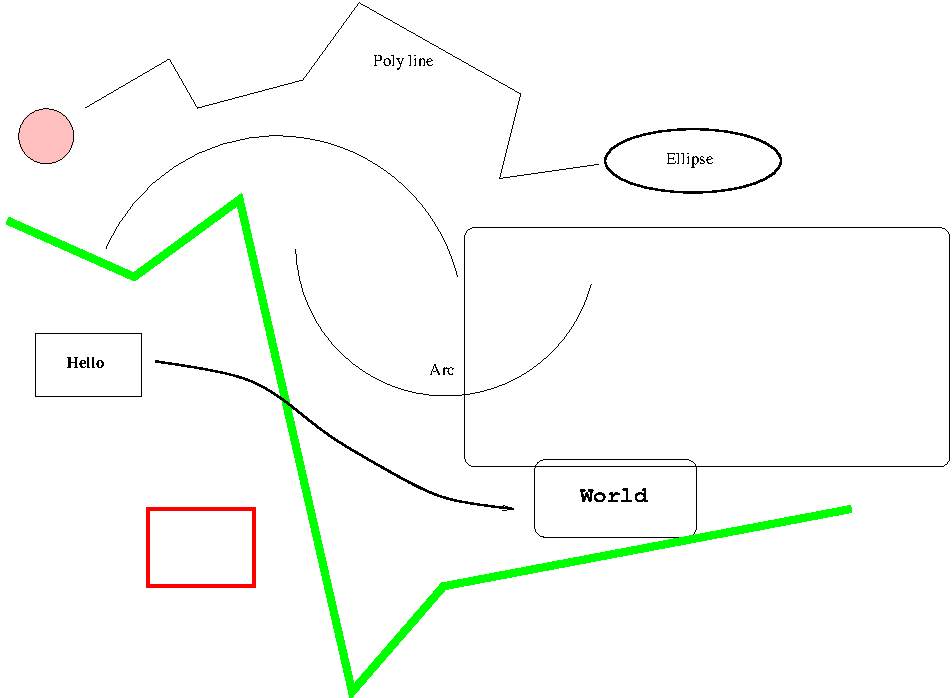
\includegraphics{figs/diagram.pdf}}
\caption{Example diagram drawn using \texttt{xfig}}
\label{xfig}
\end{figure}


\chapter{Evaluation}

\section{Printing and binding}

Use a ``duplex'' laser printer that can print on both sides to print
two copies of your dissertation. Then bind them, for example using the
comb binder in the Computer Laboratory Library.

\section{Further information}

See the Unix Tools notes at

\url{http://www.cl.cam.ac.uk/teaching/current-1/UnixTools/materials.html}


\chapter{Conclusion}

I hope that this rough guide to writing a dissertation is \LaTeX\ has
been helpful and saved you time.


%%%%%%%%%%%%%%%%%%%%%%%%%%%%%%%%%%%%%%%%%%%%%%%%%%%%%%%%%%%%%%%%%%%%%
% the bibliography
\addcontentsline{toc}{chapter}{Bibliography}
\bibliography{refs}

%%%%%%%%%%%%%%%%%%%%%%%%%%%%%%%%%%%%%%%%%%%%%%%%%%%%%%%%%%%%%%%%%%%%%
% the appendices
\appendix

\chapter{Latex source}

\section{diss.tex}
{\scriptsize\verbatiminput{diss.tex}}

\section{proposal.tex}
{\scriptsize\verbatiminput{proposal.tex}}

\chapter{Makefile}

\section{makefile}\label{makefile}
{\scriptsize\verbatiminput{makefile.txt}}

\section{refs.bib}
{\scriptsize\verbatiminput{refs.bib}}


\chapter{Project Proposal}

\documentclass[12pt]{article}

\usepackage{minted}
\usepackage{hyperref}
\usepackage{datetime}
\usepackage{datenumber}
\usepackage{advdate}
\usepackage[super]{nth}
\usepackage[margin=0.75in]{geometry}

\parindent 0pt \parskip 6pt

\newcommand\todo[1]{\textbf{TODO(kc506): #1}}
\newcommand\haskell[1]{\mintinline{haskell}{#1}}
\newcommand\monospace[1]{\mintinline{text}{#1}}

\begin{document}

\thispagestyle{empty}

\centerline{\large Computer Science Tripos: Part II Project Proposal}
\vspace{0.4in}
\centerline{\Large\bf Measuring mutual information within Neural networks}
\vspace{0.3in}

\centerline{Andrius Grabauskas, ag939}
\centerline{Robinson College}

% TODO(ag939)
\centerline{\large \textbf{date}}

\vspace{1in}

\begin{tabular}{ p{4cm} p{4.5cm} l }
{\bf Project Originator:} & Andrius Grabauskas & \\[3mm]
{\bf Project Supervisor:} & Dr.\ Damon Wischik & {\bf Signature:} \\[3mm]
{\bf Director of Studies:} & Prof.\ Alan Mycroft & {\bf Signature:} \\[3mm]
{\bf Overseers:} & Dr.\ Robert Mullins & {\bf Signature:} \\[3mm]
                 & Prof.\ Pietro Lio' & {\bf Signature:} \\[3mm]
\end{tabular}

\vspace{0.75in}

\section*{Introduction and Description of the Work}

The goal of this project is to confirm or deny the results produced by
Shwartz-ziv \& Tishby in their paper ``Opening the black box of Deep Neural
Networks via Information``\footnote{https://arxiv.org/abs/1703.00810}

The paper tackles our understating of Deep Neural Networks (DNNs). As of yet
there is no comprehensive theoretical understanding of how DNNs learn from data.
The authors proposed to measure how information travels within the DNNs layers.

They found that training of neural networks can be split into to two distinct
phases: memorization followed by the compression phase.
\begin{itemize}
  \item memorization - each layer increases information about the input and the
    label
  \item compression  - this is the generalization stage where each layer tries
    to forget details about the input while still increasing mutual information
    with the label thus improving performance of the DNN. This phase takes the
    wast majority of the training time.
\end{itemize}

They found that each layer in neural network tries to throw out unnecessary data
from the input while preserving information about the output/label. As the
network is trained each layer preserves more information about the label

The results they found were interesting but also contentious as they have not
yet provided a formal proof, just experimental data as a result there are many
peers that are cautious and sceptical of the theory.

\section*{Starting Point}

I have watched a talk that Prof.\ Tishby gave on this topic at Yandex, no other
preparation was done. 

\section*{Resources Required}

I will use my own laptop to train and evaluate the neural networks as I expect
them to be small given the difficulty of measuring mutual information and
entropy in neural networks.

For backups I intend to store my work on GitHub and my own personal machine. In
case my laptop breaks I will get another one or use the MCS machines.

\section*{Substance and Structure of the Project}

The aim of this project to reproduce the results provided by Prof.\ Tishby and
his colleagues. The intention of my work is to help settle the debate surrounding the
topic either strengthening the arguments in favour of the theory in case my
results are inline with the aforementioned results or encourage discussion in
case my results contradict the theory.

My work will require me to learn a great deal of Information theory and DNN
theory. In order for my results to be valid.

One of the more contentious parts of my project will be measuring mutual
information between the input a layer in the DNN and the label. Mutual
information is known to be tricky to measure when it comes to Continuous random
variables.

Will need to use Python to train the neural networks and GNUplot or alternative
to plot the results.

\section*{Success Criteria}

Confirm or deny the results produced in``Opening the black box of Deep Neural
Networks via Information`` paper on the same dataset as the paper. In order to do
that I will need to:

\begin{itemize}
  \item Train a neural network
  \item Measure the mutual information between input the layers and the label.
  \item Analyze the results
\end{itemize}

\section*{Extensions}

The dataset used in the original paper is very non-standard so it would be very
interesting to see how the theory holds up when we use it with different
datasets.

Different datasets will most likely need different ways to approximate mutual
information between layers.

\section*{Schedule}

% Set start date to 15th October 2018
\ThisYear{2018}\ThisMonth{10}\ThisDay{15}

% Specify date format like "15th Oct"
\newdateformat{datefmt}{\nth{\THEDAY} \shortmonthname[\THEMONTH]}

% Force advdate commands to change the global "today" instance, not the local one
\makeatletter
\renewcommand\AdvanceDate[1][\@ne]{\global\advance\day#1 \FixDate}
\renewcommand\FixDate{%
  \FixMonth \is@LeapYear
  \l@@p \global\ifnum\day<1 \Pr@vD@y \repeat
  \l@@p \M@s\m@sic \global\ifnum\day>\M@s \N@xtD@y \repeat
}
\renewcommand\FixMonth{%
  \L@@p \global\ifnum\month<1 \global\advance\year\m@ne \global\advance\month12 \is@LeapYear \repeat
  \L@@p \global\ifnum\month>12 \global\advance\year\@ne \global\advance\month-12 \is@LeapYear \repeat}
\def\Pr@vD@y{%
  \global\ifnum\day<-366
    \global\ifnum\month>2
      \global\advance\day\r@k \global\advance\year\m@ne \is@LeapYear
    \else
      \global\advance\year\m@ne \is@LeapYear \advance\day\r@k
    \fi
  \else
    \global\advance\month\m@ne \FixMonth
    \global\advance\day\m@sic
  \fi}
\def\N@xtD@y{%
  \global\ifnum\day>366
    \global\ifnum\month>2
      \global\advance\year\@ne \is@LeapYear \global\advance\day-\r@k
    \else
      \global\advance\day-\r@k \global\advance\year\@ne \is@LeapYear
    \fi
  \else
    \global\advance\day-\M@s \global\advance\month\@ne \FixMonth
  \fi}
\makeatother

% Output eg. boldface "15th Oct - 29th Oct" when called.
\newcommand{\daterange}[1]{%
    \textbf{\datefmt\today}
    \textbf{--}
    \AdvanceDate[#1]\relax
    \AdvanceDate[-1]\relax
    \textbf{\datefmt\today}
    \AdvanceDate[1]\relax
}

\begin{itemize}
  \item {
      \daterange{42}

      Preliminary reading and examining code written provided by Prof.\ Tishby
  } \item {
      \daterange{28}

      Reproduce the Papers results on the original dataset.
  } \item {
      \daterange{14}

      Examine result and produce graphs.
  } \item {
      \daterange{42}

      Test the theory on additional datasets 
  } \item {
      \daterange{28}

      Final write up of the thesis
  }
\end{itemize}

\end{document}


\end{document}
